% 
% NTHU Template
% 2014 Yao Wei
%
% This file is licensed under CC0.
% https://creativecommons.org/publicdomain/zero/1.0/
%

\documentclass[12pt]{article}

% Lint
\RequirePackage[l2tabu, orthodox]{nag}

% Fonts
\usepackage{mathptmx}
\usepackage[T1]{fontenc}
\usepackage{CJKutf8}

% Layout
\usepackage[a4paper, top=2.54cm, bottom=2.54cm, left=3.17cm, right=2.54cm]{geometry}
\usepackage{abstract}

% Paragraph
\usepackage{indentfirst}
\usepackage{setspace}

\usepackage{tabularx}

% Watermarks
\usepackage{wallpaper}
\CenterWallPaper{.18}{./assets/nthu_watermark.eps}
\setlength{\wpXoffset}{0.315cm}

% Citations

\usepackage[backend=bibtex,sorting=none,maxcitenames=2,maxbibnames=3,hyperref=true,block=none]{biblatex}
\bibliography{thesis}
\renewbibmacro{in:}{}

% Figures
\usepackage{float}
\usepackage{subcaption}
\usepackage{rotating}

% algo
\usepackage{algorithm}
\usepackage{algorithmicx}
\usepackage{algpseudocode}
\renewcommand{\algorithmicrequire}{\textbf{Input:}}
\renewcommand{\algorithmicensure}{\textbf{Output:}}
%\usepackage{amsmath}


\begin{document}
\begin{CJK}{UTF8}{bkai}

\begin{titlepage}
\begin{center}
\Huge 國~立~清~華~大~學 \\ [1.5ex]
\Huge \underline{碩~士~論~文} \\
%\Large (初稿)\\
\vspace*{10ex}
\huge 適用於異質系統架構的數位訊號處理器設計 \\
\vspace*{1ex}
\huge DeAr: An Efficient DSP Datapath Design for Heterogeneous System Architecture  \\

\null
\vfill

\Large
\begin{tabular}{r@{\centering} @{}l}
    系\ 所\ 別:~&電機工程學系碩士班\ \ \ 組別:系統組	\\ [1.5ex]
    學號姓名:~&103061568~李齊明~(Chi-Ming~Lee)      \\ [1.5ex]
    指導教授:~&許雅三~博士~(Prof.~Yarsun~Hsu)       \\
	
\end{tabular}

\vspace*{2ex}
\Large 中華民國 105 年 6 月
\end{center}
\end{titlepage}

\doublespacing
\pagenumbering{roman}
\setcounter{page}{3}
\addcontentsline{toc}{section}{Abstract}

\renewcommand{\abstractnamefont}{\normalfont\bfseries}
\renewcommand{\abstracttextfont}{\normalfont}
\setlength{\absleftindent}{0pt}
\setlength{\absrightindent}{0pt}

\begin{abstract}  % Abstract
	Will be done last.
\end{abstract}
\clearpage
\addcontentsline{toc}{section}{Acknowledgements}

\begin{center}
\textbf{Acknowledgements}
\end{center}
Acknowledgements Page
\clearpage

\singlespacing

\tableofcontents  % Table of contents
\clearpage
\addcontentsline{toc}{section}{List of Figures}
\listoffigures  % List of figures
\clearpage
\addcontentsline{toc}{section}{List of Tables}
\listoftables  % List of tables
\clearpage
\addcontentsline{toc}{section}{List of Algorithms}
\listofalgorithms  % List of tables
\clearpage

\doublespacing
%\setlength{\parskip}{12pt}

\pagenumbering{arabic}

\section{Introduction}

    \subsection{Motivation}
        As wireless communication standard evolves, the demand for digital signal processing platform that supplies computation with high-performance, high-flexibility and low-energy consumption is gaining momentum in the mobile industry. 
        Take an example of LTE-advance, which is considered to be the next mainstream mobile wireless technology, it provides 10 times higher transmission throughput than that of LTE \cite{lte}. 
        In order to achieve this enhancement, strategies such as scaling up MIMO system and permitting carrier aggregation \cite{carrier} that require more sophisticated arithmetics are adopted in LTE-advance.
        Moreover, these algorithms used in LTE-advance demodulation will still change frequently with the protocol specification.
        Consequently, both energy efficiency and flexibility become crucial considerations in the filed of digital signal processor implementation. 
        However, VLIW and ASIP, which have been popular choices of state-of-the-art digital signal processor (DSP) micro-architecture, serve as two extremes cases for hardware designers who would like to trade-off between flexibility and energy efficiency. 
        VLIW gains good flexibility by allocating each functional unit dedicated control signals and ports on register file that result in significant power dissipation, so it could work orthogonally with each other; 
        On the contrary, ASIP benefits from optimized data-path for the specific ISA or algorithm by sacrificing its flexibility so good energy efficiency is achieved. 
        Consequently, improving energy efficiency while keeping hardware flexibility for DSP on mobile devices becomes a challenge.	\\

        On the other hand, heterogeneous computing, which is referred to systems equipped with multiple types of processors, has opened a new era for digital signal processing. 
        Such an integration of different processors gains performance improvement by taking advantage of particular processing activities to handle certain types of tasks.
        Nowadays, a digital signal processing platform typically contains a CPU that handles control intensive tasks and a DSP that perform computation intensive ones.
        Nevertheless, in such heterogeneous DSP platforms, there is still a drawback owing to the communication latency between processors. 
        Frequent data transfer and task dispatching control between DSP and CPU lead to a  bottleneck of performance. 
        As a result, HSA foundation, found by AMD, ARM, MediaTek, etc, propose a new standard for heterogeneous computing, HSA system specification \cite{systemspec}, to address the problem. 
        The standard creates concepts of unified memory space and architectural queuing language that alleviate burdens on data transfer and task dispatching, becoming the potential mainstream of computer architecture in the future \cite{mainstream}.

    \subsection{Goal and Contribution}
        To improve performance and energy efficiency as well as maintain flexibility for digital signal processing platforms, 
        we present DeAr: A Dual-thread Architecture design for DSP datapath that combines advantages of both VLIW and TTA.
        We also illustrate a framework which integrates DeAr with HSA platforms, which are able to reduce communication overhead between CPU and DSP. 
        Prominent features of DeAr include:
        \begin{itemize}
            \item The VLIW-style datapath enables two threads to execute concurrently. High operations per cycle (OPC) can be achieved with proper compiler scheduling.
            \item TTA-style transport-triggered scheduling aggressively forwards data from accumulators to functional units. Unnecessary data write back (WB) can be avoided so energy dissipation in register file is consequently reduced.
            \item Banked organization of register file eliminates redundant connections from ports to registers. Compared with the conventional centralized organization, both power consumption and circuit area are saved.
            \item Register file access is regularized to a queue/stack operation (i.e. push or pop) instead of conventional random access, which requires more bits to specify a register address. Density of VLIW-style code can be improved.
            \item DeAr is suitable for clustering and it can be scaled up to SIMD or vector-processing architectures to meet the throughput requirement.
        \end{itemize}
        In addition, to evaluate DeAr with existing architectures, we selected several classical DSP kernels \cite{dspstone} \cite{bdti} as the benchmark and use the UMC 65nm CMOS technology to implement the hardware.

        The main contribution of this work is achieve at two levels: micro-architecture and HSA level. 
        On the micro-architecture side, with equal resources of functional unit and register file, DeAr outperformed by 30\% in MOPS\/mW and improve 50\% in code density while remaining competitive computational throughput, compared with the conventional VLIW architecture.
        On the HSA side, we present a completed code generation flow for DeAr which meets the requirements from HSA standard, and illustrate a system framework for exploiting the power of DeAr in an HSA platform.
 
    \subsection{Organization}
        The remainder of this thesis is organized as follows: In Chapter 2, we briefly review work related to our architecture. In Chapter 3, we introduces background knowledge about this work. In Chapter 4, we look into the details of the proposed design. In Chapter 5, we provide experimental results that demonstrate the capabilities of this architecture. Finally, Chapter 6 present conclusions and future work of the thesis.

\newpage

\section{Related Work}
    In the stream of DSP design, many studies have been conducted on register file (RF) organization as it becomes the dominating factor of cycle time, power consumption and chip area \cite{register}.
    Rixner \textit{et al.} indicated that, for conventional centralized organization, the cost grows significantly with the number of functional units (FUs) \cite{register}, causing a challenge for designing VLIW DSP.
    A straightforward solution is partitioning the centralized RF into several parts, each of which serves specific FUs, such as \cite{cluster}.
    Studies like \cite{synzen} and \cite{dsplite} went even further by discarding the centralized RF and allocating each FU a dedicated one, which is also known as distributed RF organization.
    However, dividing RF leads to more complicated compiler design and overhead of inter-RF data transport.
    In addition, above approaches still suffer from poor code density, which is an inherent problem from the VLIW architecture.
    \\
    Some approaches avoided the aforementioned cost growth by customizing the data-path and limiting the number of ports on RF.
    Ou \textit{et al.} proposed composite FUs for DSP, which cascade FUs with a specific order and demand fewer ports on RF \cite{cascade} \cite{hearaid}.
    Similar techniques are often applied to ASIP design but they usually lack flexibility to target general purposes.
    There are further researches that achieve power reduction on RF by minimizing the number of accesses to it.
    Chen \textit{et al.} proposed a simulated-annealing based scheduling that aggressively forwards data from FU outputs to inputs instead of accessing RF \cite{multistage}.
    \cite{move} presented a processor framework: MOVE, which features the separation of data transport and operation in the data-path. 
    The user can program the bypass network in MOVE, and avoid most of accesses to RF by clever data transport.
    Such an architecture that manipulates data transport usually refers to transport-triggered architecture (TTA).
    The Work from Lama \textit{et al.} \cite{ttagpu} also demonstrated a framework that takes the advantage of TTA in graphic processing unit (GPU), and this idea is a potential alternative for DSP design.
    \\
    On the other hand, one may notices that none of the above implementations adopts HSA \cite{systemspec}, which is a promising standard for embedded DSP platforms.
    So far, most of studies on HSA focus on the integration of CPU and GPU. \cite{hsaemu} presented a full system emulator for HSA platforms that include CPUs and GPUs.
    Beyond emulation, \cite{hsacyc} further illustrated a cycle-accurate HSA simulator that integrates QEMU and GPGPU-sim \cite{gpgpusim}.
    To the best of our knowledge, little or no research has been performed to apply the standard to DSP platforms.

\newpage

\section{Background}

    \subsection{Evolution of Digital Signal Processors}
        A digital signal processor (DSP) is an optimized computer design that aims at accelerating digital signal processing, such as baseband demodulation or video codec.
        In principle, a programmer extracts routines or algorithms from applications and accelerates them with a DSP.
        Such pieces of code that executed by DSPs are also referred to DSP kernels.
        Unlike general purpose computers, which usually feature powerful ISA and novel branch predictors that help them dealing with control intensive tasks very well,
        DSPs simply focus on computation intensive tasks delivered by another unit (general purpose processor, analog to digital converter, etc.), 
        and thus its hardware can be simplified and optimized for better power efficiency, which enable them to be widely used in mobile devices and embedded systems.
        \\
        The single-issue reduced instruction set computer (RISC), introduced in 1980s \cite{risc}, becomes a popular template for DSP owing to its simplicity.
        The key concept of RISC is designing an ISA with primitive and orthogonal instructions which demand simpler datapath.
        By taking the advantage of the regularity in the datapath, pipelining technique can thus be adopt to achieve the application requirement.
        However, two drawbacks still exist in single-issue RISC. 
        The first is lack of instruction-level parallelism (ILP). 
        Functional units are not able to work concurrently due to the limitation of the single-issue datapath.
        This can be resolved by designing a multi-issue datapath with either hardware (i.e., superscalar) or software scheduling (i.e., VLIW).
        In the field of DSP design, adopting the VLIW architecture is a preferable strategy, 
        because hardware simplicity matters than portability and many optimization approaches can be applied in compilation stages. 
        Figure~\ref{fig:vliw} illustrates a basic VLIW datapah, where multiple instructions can be executed at a cycle.
        The number of ports on RF is scaled up with the issue-width, and the compiler is responsible for performing static scheduling to avoid resources conflict among operations.
        \begin{figure}[!ht] 
            \caption{A basic VLIW datapah}
            \centering
            \includegraphics[width=0.5\textwidth]{./figs/vliw.eps}
            \label{fig:vliw}
        \end{figure}
        \\
        The second drawback is plenty of redundant write back (WB). 
        In digital signal processing, intermediate results are often read exactly once, which implies lots of RF storage of them is redundant.
        Several approaches have been proposed to address this issue.
        Figure~\ref{fig:cascade} shows a datapath with a customized composite FU that cascades primitive FUs. 
        Intermediate results can be forwarded from one to its follower with an optimized order which targets specific applications.
        Processor with such customization is referred to application-specific instruction set processor (ASIP).
        \begin{figure}[!ht] 
            \caption{A datapath with a composite functional unit}
            \centering
            \includegraphics[width=0.6\textwidth]{./figs/cascade.eps}
            \label{fig:cascade}
        \end{figure}
        \\
        Another approach that enables forwarding mechanism even further is shown in Figure~\ref{fig:tta}, where FUs, RF and load/store units are linked by an interconnection network (ICN).
        Such an architecture makes a significant distinction from RISC because only a "move" instruction is needed. 
        All computation can be completed by moving operands on the interconnection network, avoiding WB as much as possible.

        \begin{figure}[!ht] 
            \caption{Transport triggered architecutre (TTA)}
            \centering
            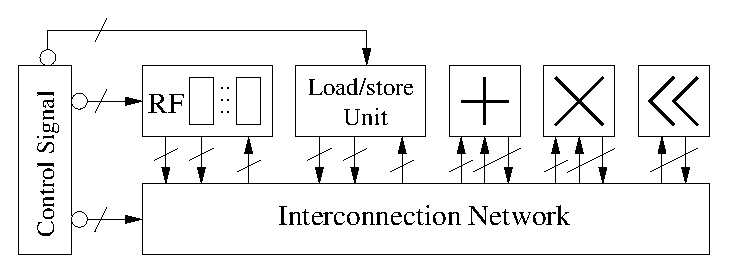
\includegraphics[width=0.8\textwidth]{./figs/tta.eps}
            \label{fig:tta}
        \end{figure}
      
        %\subsubsection{Application-Specific Instruction Set Processor}
        %\subsubsection{Very Long Instruction Word Processor}
        %\subsubsection{Transport-Triggered Architecture}

    \subsection{Register Files Organization}
        %\subsubsection{Centralized Register Files}
        %\subsubsection{Banked Register Files}
        %\subsubsection{Clustered Register Files}
        %\subsubsection{Distributed Register Files}
    \subsection{Heterogeneous System Architecture}
        \subsubsection{System Specification}
        \subsubsection{Software Stack}

\section{Design and Implementation}
    \subsection{System Overview}
    \subsection{Micro-architecture Design}
        Figure~\ref{fig:micro} demonstrates the micro-architecture of DeAr datapath.
        \begin{figure}[!ht] 
            \caption{Micro-architecture of DeAr}
            \centering
            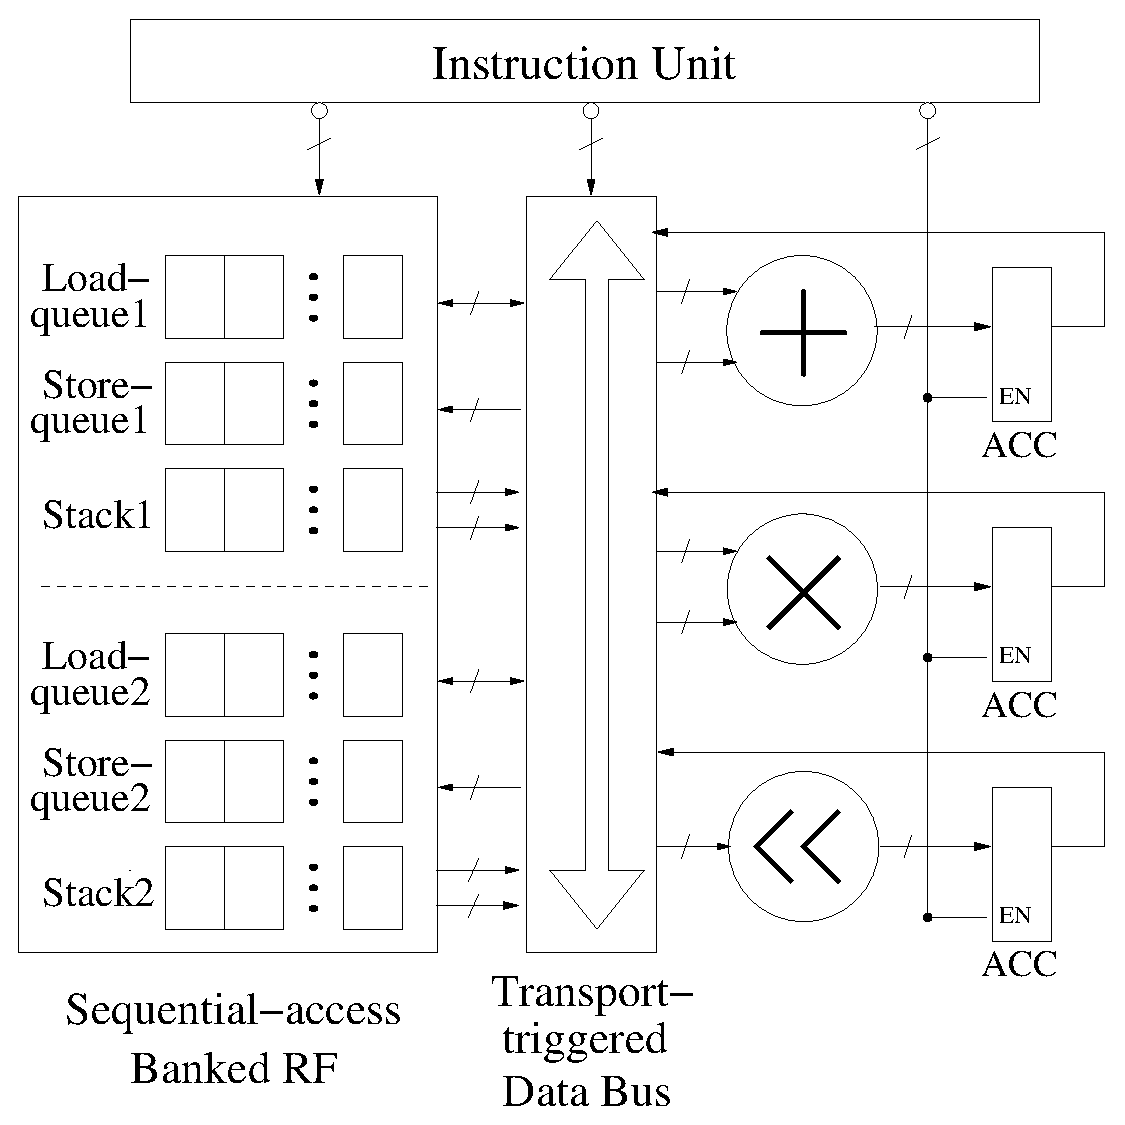
\includegraphics[width=0.8\textwidth]{./figs/micro.eps}
            \label{fig:micro}
        \end{figure}
    \subsection{Software Design}
        \subsubsection{Software framework for DeAr}
            To fully exploit the power of DeAr, we also present a completed code generation flow including compilation, scheduling and optimization.
            Algorithm~\ref{alg:framework} provides an overview of the software framework for DeAr. 
            The user only need to provide DSP kernel code written in OpenCL and a flag which determines the optimization level as the input.
            With CLOC \cite{cloc} tool provided by HSAfoundation, the kernel code is converted to standardized HSAIL, $H$, as shown in Line~\ref{line:tohsail}.
            Next, in Line~\ref{line:tran}, we run the transformation $T$ (elaborated in \ref{sec:trans}) on $H$ and obtain a particular data structure $\bar{G}$ that represent the DSP kernel.
            After that, from Line~\ref{line:optstart} to Line~\ref{line:optend}, we perform the key part of DeAr software, operation scheduling and optimization (elaborated in \ref{sec:sando}).
            The optimization flag $\lambda$ in Line~\ref{line:forlambda} determines the number of iterations to be used.
            For each iteration, the scheduler exhausts heuristics in $\bar{G}$ which optimize the cycle and WB counts, and it schedules operations with a limited randomness.
            Finally, the scheduler select the scheduling result with the least cycle count, $C_{golden}$ among iterations and generates the final code $X_{golden}$ for DeAr as the output.

            %%%%%%%%%%%% framework algo 
            \begin{algorithm}[h]
              \caption{Software framework for DeAr}
              \begin{algorithmic}[1]
                    \Require 
                        High-level DSP kernel code in OpenCL, Optimization flag $\lambda$
                    \Ensure 
                        Binary code of DeAr

                  \State Convert the kernel code to HSAIL, expressed by $H$;
                  \label{line:tohsail}
                  %\State Perform SSA transformation on HSAIL;
                  %\label{tossa}
                  %\State Convert SSA code to DFG, $G = ( V_{op} , E_{op} )$, where $V_{op}$ is the set of operations and $E_{op}$ is the set of their dependencies;
                  %\label{todfg}
                  %\State Perform hierarchization on $G$, and get $\bar{G} = ( V_{bt} , E_{bt} )$, where $V_{bt}$ is a set of binary trees and $E_{bt}$ is the set of their dependencies;
                  \State Perform the transformation $T$ on $H$, and obtain $T(H) = \bar{G}$ which holds scheduling heuristics of the kernel;
                  \label{line:tran}
                  \State $C_{golden} \leftarrow  \infty$;
                  \label{line:optstart}
                  \For {$i=1$ to $f(\lambda)$}
                    \label{line:forlambda}
                    \State Schedule operations in $\bar{G}$ and get binary code $X_i$ and its total cycle count $C_i$;
                    \If {$C_i < C_{golden}$}
                      \State $C_{golden} \leftarrow C_i$;
                      \State $X_{golden} \leftarrow X_i$;
                    \EndIf
                  \EndFor
                  \State Return $X_{golden}$;
                  \label{line:optend}
              \end{algorithmic}
              \label{alg:framework}
            \end{algorithm}
            %%%%%%%%%%%%%%%%%%%%%%%%%%%%5


        
        \subsubsection{Transformation}
        \label{sec:trans}
        \subsubsection{Scheduling and Optimization}
        Algorithm~\ref{alg:inter}
        \label{sec:sando}

\begin{algorithm}[h]
  \caption{Inter-tree scheduling}
  \begin{algorithmic}[1]
        \Require 
            Binary trees set of a DFG, ;    
        \Ensure 
            Uncompleted binary code; Rest of the last tree;
    \For{each $i\in [1,9]$}
      \State initialize a tree $T_{i}$ with only a leaf (the root);
      \State $T=T\cup T_{i};$
    \EndFor
    \ForAll {$c$ such that $c\in RecentMBatch(E_{n-1})$}
      \label{code:TrainBase:getc}
      \State $T=T\cup PosSample(c)$;
      \label{code:TrainBase:pos}
    \EndFor;
    \For{$i=1$; $i<n$; $i++$ }
      \State $//$ Your source here;
    \EndFor
    \For{$i=1$ to $n$}
      \State $//$ Your source here;
    \EndFor
    \State $//$ Reusing recent base classifiers.
    \label{code:recentStart}
    \While {$(|E_n| \leq L_1 )and( D \neq \phi)$}
      \State Selecting the most recent classifier $c_i$ from $D$;
      \State $D=D-c_i$;
      \State $E_n=E_n+c_i$;
    \EndWhile
    \label{code:recentEnd}
  \end{algorithmic}
  \label{alg:inter}
\end{algorithm}


\section{Performance Evaluation}
    \subsection{Operation per Cycle}
    \subsection{Write back per Operation}
    \subsection{MOPS vs Area}
    \subsection{MOPS vs Energy}

\section{Conclusions and Future Work}

\clearpage

\addcontentsline{toc}{section}{References}
\singlespacing
%\setlength{\parskip}{0pt}

\printbibliography

\end{CJK}
\end{document}
